\documentclass{../industrial-development}
\graphicspath{{6-interaction-inside-and-outside-team/}}

\title{Команда разработчиков: взаимодействие внутри и вне команды}
\author{Смирнов Дмитрий Владиславович, ПИЭ-21 МО}
\date{}

\begin{document}

\begin{frame}
  \titlepage
\end{frame}


\section{Взаимодействие внутри команды}

\subsection{Вертикальная форма взаимодействия сотрудников}

\begin{frame} \frametitle{Вертикальная форма взаимодействия сотрудников}
  \begin{block}{Что это такое?}
 Вертикальная форма взаимодействий имеет структуру подчиненности от верхнего уровня к нижнему. Существует четко определенная цепочка командования с вертикальной организацией, и человек в верхней части организационной структуры имеет наибольшую власть. Сотрудники отчитываются перед лицом непосредственно над ними в организационной структуре. Каждый человек несет ответственность за определенную область или набор обязанностей.
  \end{block}
\end{frame}

\lecturenotes
Вертикальная (линейная) форма взаимодействия –  это простейшая форма взаимодействий иерархического типа, характеризующаяся тем, что во главе каждого звена или подразделения стоит единоличный руководитель, наделенный всем объемом полномочий и власти. 

\begin{frame} \frametitle{Пример}
  \begin{block}{Пример}
\centerline{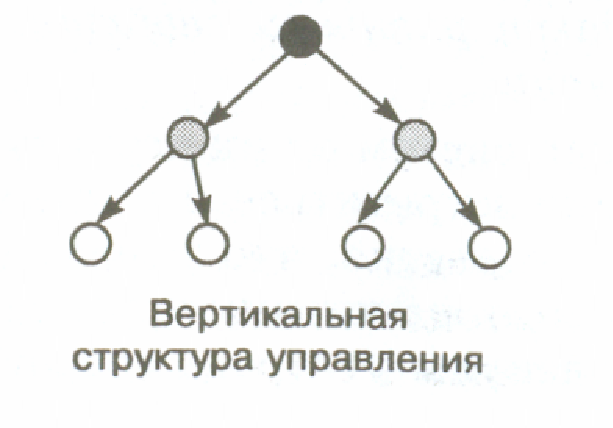
\includegraphics[width=1\textwidth]{vertical.pdf}}
  \end{block}
\end{frame}

\lecturenotes
Пример вертикальной формы взаимодейтсвия в ИТ компании:
1ый уровень - руководитель компании
2ой уровень - исполнительный директор (отвечает за ведение проектов) и коммерческий директор (отвечает за продажи)
3й уровень - менеджеры проектов и менеджеры продаж.

Также можно рассмотреть другой вариант данной формы взаимодействия в ИТ команде:
1ый уровень -  технический директор
2ой уровень -  руководитель отдела разработки и руководитель отдела тестирования
3ий уровень - программисты и тестировщики


\begin{frame} \frametitle{Преимущества}
  \begin{block}{Преимущества вертикальной формы}
  \end{block}
  
  \begin{itemize}
  \item удобное распределение задач
  \item простота управления
  \item имеется возможность роста по карьерной лестнице
  \item четко выраженная ответственность
  \item высокий уровень специализации профессиональной деятельности и компетентности специалистов

  \end{itemize}
\end{frame}


\begin{frame} \frametitle{Недостатки}
  \begin{block}{Недостатки вертикальной формы}
  \end{block}
  
  \begin{itemize}
  \item медленное общение между отделами и сотрудниками
  \item концентрация власти на верхнем уровне управления
  \item большая физическая и моральная нагрузка на руководителей
  \item в такой структуре низшее звено может чувствовать себя подавленным или чувстовавать, что их вклад не важен
  \end{itemize}
\end{frame}

\subsection{Горизонтальная форма взаимодействия сотрудников}

\begin{frame} \frametitle{Горизонтальная форма взаимодействия сотрудников}
  \begin{block}{Что это такое?}
Горизонтальные связи — это связи между двумя или более равными по положению в иерархии или статусу членами команды. Каждый сотрудник имеет аналогичный вклад в то, как работает организация. Они могут выполнять множество различных функций и могут отчитываться перед несколькими руководителями, а не одним начальником. Например, руководители проектов или руководители групп отчитываются перед командой руководителей, причем члены каждой команды по существу равны с точки зрения власти.
  \end{block}
\end{frame}

\begin{frame} \frametitle{Пример}
  \begin{block}{Пример}
\centerline{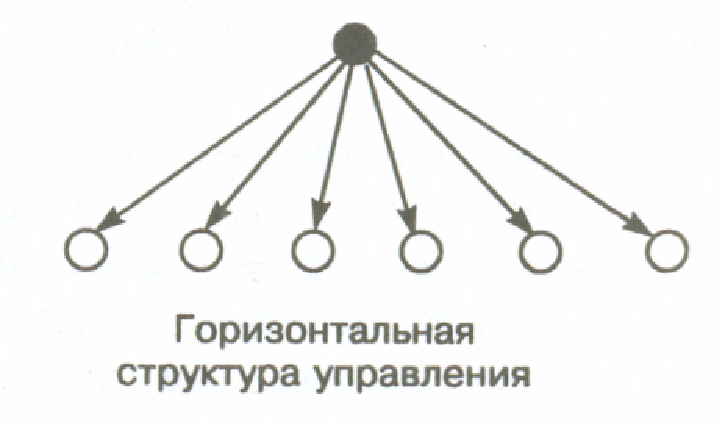
\includegraphics[width=1\textwidth]{horizontal.pdf}}
  \end{block}
\end{frame}

\lecturenotes
Пример горизонтальной формы взаимодейтсвия в ИТ компании:
1ый уровень - главный менеджер проектов
2ой уровень - менеджеры проектов

Также можно рассмотреть другой вариант данной формы взаимодействия в ИТ команде:
1ый уровень -  ведущий дизайнер
2ой уровень - дизайнеры

\begin{frame} \frametitle{Преимущества}
  \begin{block}{Преимущества горизонтальной формы}
  \end{block}
  
  \begin{itemize}
  \item высокий моральный дух сотрудников, поскольку они имеют больше полномочий на принятие решений
  \item поскольку сотрудники  имеют право принимать свои собственные решения, сотрудничество с клиентами происходит быстрее
  \item сотрудники имеют открытый контакт друг с другом и более доступны для принятия совместных решений
  \end{itemize}
\end{frame}

\subsection{Матричная форма взаимодействия сотрудников}

\begin{frame} \frametitle{Матричная форма взаимодействия сотрудников}
  \begin{block}{Что это такое?}
Матричная структура представляет собой комбинацию двух видов разделения: по функциям и по продукту. Она построенна на основе принципа двойного подчинения исполнителей: с одной стороны, непосредственному руководителю функционального подразделения, которое предоставляет персонал руководителю проекта, с другой стороны  - руководителю временной группы, который наделен необходимыми полномочиями для осуществления процеса управления и несет ответственность за сроки и ресурсы.
  \end{block}
\end{frame}

\begin{frame} \frametitle{Пример}
  \begin{block}{Пример}
\centerline{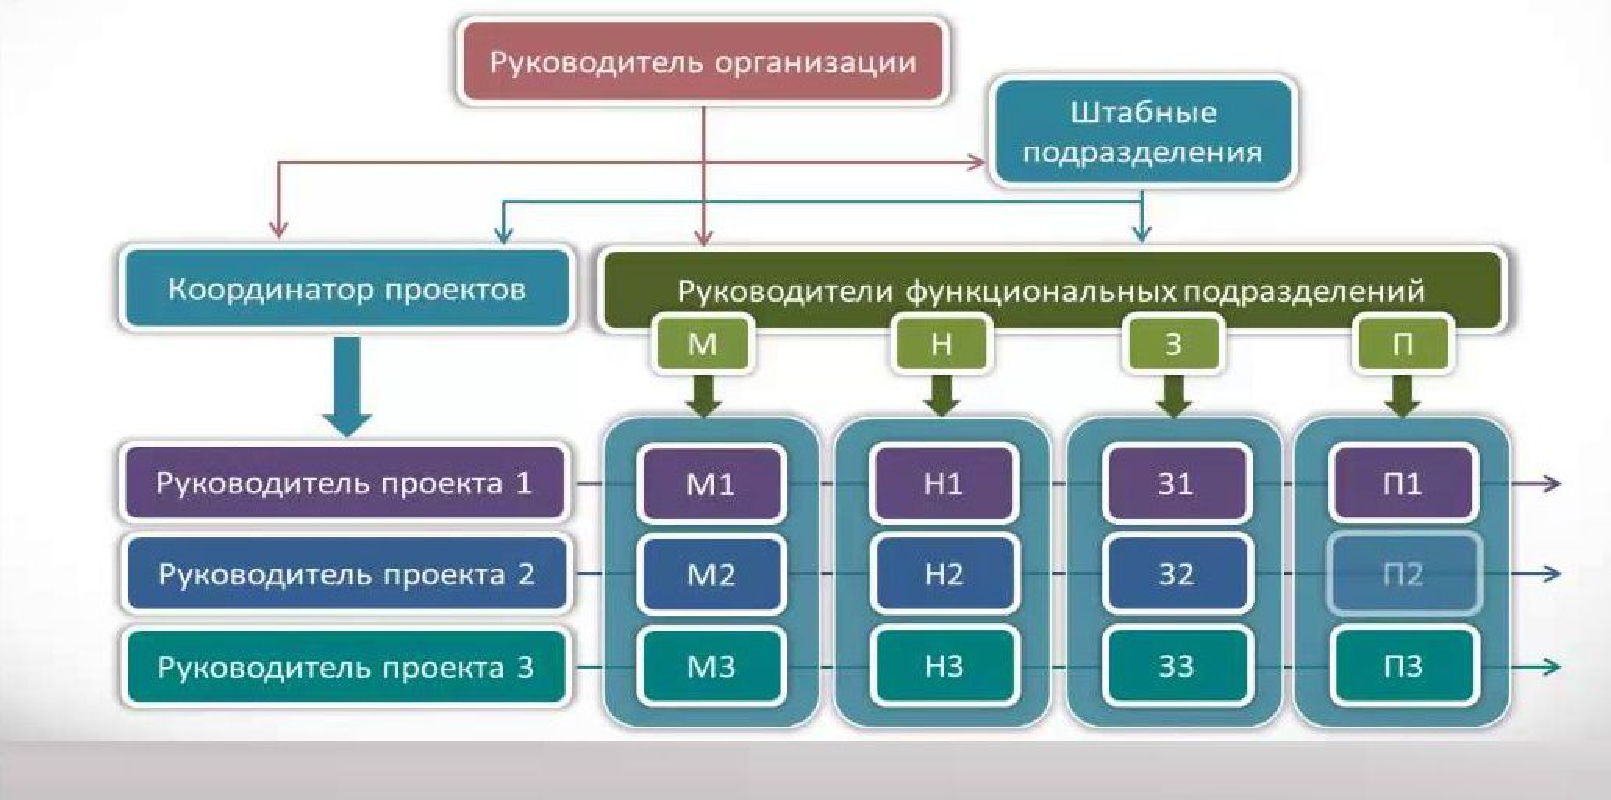
\includegraphics[width=1\textwidth]{matrix.pdf}}
  \end{block}
\end{frame}

\lecturenotes
Матричные структуры охватывают не всю организацию, а лишь ее часть. Причем успех в значительной мере зависит от того, в какой степени руководители проектов обладают профессиональными качествами менеджеров и способны выступить в проектной группе в роли лидеров.
Руководители проектов в матричной структуре отвечают в целом за интеграцию всех видов деятельности и ресурсов, относящихся к данному проекту. Для того, чтобы они смогли добиться этого, все материальные и финансовые ресурсы по данному проекту передаются в их полное распоряжение. Руководители проектов сохраняют за собой право определять приоритетность и сроки решения той или иной задачи, в то время как руководители структурных подразделений могут лишь выбирать конкретного исполнителя и методику решения.
Матричные формы взаимодеййствий очень активно используются в IT  командах

\begin{frame} \frametitle{Преимущества}
  \begin{block}{Преимущества матричной формы}
  \end{block}
  
  \begin{itemize}
  \item сокращение нагрузки на руководителей высшего уровня управления 
  \item получение высококачественных результатов по большому количеству проектов
  \item активизация деятельности руководителей и работников управленческого аппарата в результате формирования проектных команд, активно взаимодействующих с функциональными подразделениями
  \item усиление личной ответственности конкретного руководителя за его проект
  \end{itemize}
\end{frame}

\begin{frame} \frametitle{Преимущества}
  \begin{block}{Преимущества матричной формы}
  \end{block}
  
  \begin{itemize}
 \item достижение большей гибкости выполнения работ по всем проектам
 \item эффективное использование ресурсов
 \item гибкость и адаптивность к нагрузкам по проектам
 \item четкое разграничение по проектам
 \item проект находится в центре внимания - клиент доволен
  \end{itemize}
\end{frame}

\lecturenotes
Преимущества матричной формы
- Сокращение нагрузки на руководителей высшего уровня управления путем передачи полномочий принятия решений на средний уровень при сохранении единства координации и контроля за ключевыми решениями на высшем уровне
- Получение высококачественных результатов по большому количеству проектов
- Активизация деятельности руководителей и работников управленческого аппарата в результате формирования проектных команд, активно взаимодействующих с функциональными подразделениями
- Усиление личной ответственности конкретного руководителя как за проект в целом, так и за его элементы (в частности за трудовые ресурсы)
- Достижение большей гибкости выполнения работ по всем проектам
- Эффективное использование ресурсов
- Гибкость и адаптивность к нагрузкам по проектам
- Четкое разграничение по проектам
- Проект находится в центре внимания - клиент доволен

\begin{frame} \frametitle{Недостатки}
  \begin{block}{Недостатки матричной формы}
  \end{block}
  
  \begin{itemize}
  \item сложность матричной структуры для практической реализации
  \item возникновение конфликтов
  \item порождается двусмысленность роли исполнителя и его руководителей
  \item борьба за власть
  \item наблюдается частичное дублирование функций
  \item несвоевременно принимаются управленческие решения
  \item нарушается традиционная система взаимосвязей между подразделениями
  \item отсутствует полноценный контроль по проектам
  \item сложность координации проектных групп
  \item проблемы  с определением приоритетов по проектам
  \end{itemize}
\end{frame}

\lecturenotes
Недостатки матричной формы
- Сложность матричной структуры для практической реализации, для ее внедрения необходима длительная подготовка работников и соответствующая организационная культура
- В связи с системой двойного подчинения подрывается принцип единоначалия, что часто приводит к конфликтам между менеджерами функиональных подразделений и управляющими проектов, между проектной и функциональной структурами. Появляется возможность острых противоречий между сторонами матрицы.
- В рамках этой структуры порождается двусмысленность роли исполнителя и его руководителей, что создает напряжение в отношениях между членами трудового коллектива компании
- Характерна борьба за власть, так как в ее рамках четко не определены властные полномочия
- Наблюдается частичное дублирование функций
- Несвоевременно принимаются управленческие решени - характерно групповое принятие решений
- Нарушается традиционная система взаимосвязей между подразделениями
- Затрудняется и практически отсутствует полноценный контроль по проектам
- Сложность координации проектных групп
- Каждая из проектных групп будет тянуть одеяло на себя – возникнут проблемы  с определением приоритетов

\section{Взаимодействие с заказчиками}

\begin{frame} \frametitle{Выстраивание отношений с заказчиками}
  \begin{block}{Выстраивание отношений с заказчиками}
Правильное выстраивание взаимоотношений с заказчиком - очень серьезная доля успеха проекта. 
  \end{block}

\begin{itemize}
 \item знакомство с клиентом
 \item установление взаимоотношений
 \item составление договора и ТЗ
 \item информирование заказчика о технологии ведения проекта
 \item сбор команды на проект 
 \item старт проекта 
 \item мониторинг хода работы по проекту
 \item сдача работ
 \item постпроектные взаимоотношения
  \end{itemize}
\end{frame}

\lecturenotes
1. Знакомство с клиентом
  - сбор информации о компании
  -  выяснение потребностей клиента
  - предоставление оценочной стоимости за данную работу
 -  выяснение, готов ли клиент столько платить (естественно сразу никто не назовет конкретных сумм, но если проект приблизительно оценивается в 3-5 миллионов, а потенциальный заказчик считает, что миллион –  это очень много, то, наверное, у вас с ним ничего не получится)
  - формирование вывода: подходит ли такой клиент Вам или нет
2. Установление взаимоотношений
3. Составление договора и ТЗ.
4. Информирование заказчика о технологии ведения проекта
 - какие технологии будут использоваться
 - кто за что отвечает
 - кто что делает
 - для чего делаются те или иные действия
 Это необходимо для решения проблемных вопросов о задержках сроков или изменения бюджета.
5. Далее следует собрать команду на проект: назначить менеджера проекта и определиться с командой разработчиков.
6. Старт проекта.
7. Мониторинг хода работы по проекту. 
На данном этапе у клиента могут появиться желания по доработке/изменению программы или какого-либо функционала. Чтобы избежать конфликта с клиентом, менеджеру проекта приходится объяснять, что эти правки могут отразиться на сроках сдачи продукта, а также может измениться его стоимость, поскольку данные правки займут n-ое количество часов и их надо будет оплатить. В конце концов, клиент с нами соглашается и либо отказывается от своего пожелания, либо оплачивает дополнительные часы. 
8. Сдача работ.
На данном этапе следует добиться сдачи работ в полном соответствии с правилами, установленными в соответствующих документах, которые подписанным клиентом.
9. Постпроектные отношения. 
На данном этапе стоит добиться заключения договора на техническое обслуживания продукта.

\section{Проблемы взаимодействия с подрядчиками}
\begin{frame} \frametitle{Проблемы взаимодействий с подрядчиками}
  \begin{block}{Проблемы взаимодействий с подрядчиками}
  \end{block}

\begin{itemize}
 \item срыв сроков 
 \item некачественная работа
 \item невнимание к ТЗ
 \item отсутствие требуемого опыта
 \item применение старых технологий
 \item снижение мотивации
 \item неспособность быстро решить возникшую проблему
  \end{itemize}
\end{frame}

\lecturenotes
Если в штате компании не хватает программистов, и имеется большое количество задач по проектам, то можно нанять подрядчика. В качестве его могут выступать как и фрилансеры, так и другие компании. Конечно же, в этом все равно есть определенные риски, и поэтому следует выбирать подрядчика очень внимательно. 

\begin{thebibliography}{99}
\end{thebibliography}

\end{document}
